\documentclass[bachelor, och, referat]{SCWorks}
% параметр - тип обучения - одно из значений:
%    spec     - специальность
%    bachelor - бакалавриат (по умолчанию)
%    master   - магистратура
% параметр - форма обучения - одно из значений:
%    och   - очное (по умолчанию)
%    zaoch - заочное
% параметр - тип работы - одно из значений:
%    referat    - реферат
%    coursework - курсовая работа (по умолчанию)
%    diploma    - дипломная работа
%    pract      - отчет по практике
% параметр - включение шрифта
%    times    - включение шрифта Times New Roman (если установлен)
%               по умолчанию выключен
\usepackage{subfigure}
\usepackage{tikz,pgfplots}
\pgfplotsset{compat=1.5}
\usepackage{float}

%\usepackage{titlesec}
\setcounter{secnumdepth}{4}
%\titleformat{\paragraph}
%{\normalfont\normalsize}{\theparagraph}{1em}{}
%\titlespacing*{\paragraph}
%{35.5pt}{3.25ex plus 1ex minus .2ex}{1.5ex plus .2ex}

\titleformat{\paragraph}[block]
{\hspace{1.25cm}\normalfont}
{\theparagraph}{1ex}{}
\titlespacing{\paragraph}
{0cm}{2ex plus 1ex minus .2ex}{.4ex plus.2ex}

% --------------------------------------------------------------------------%
\usepackage[T2A]{fontenc}
\usepackage[utf8]{inputenc}
\usepackage{graphicx}
\graphicspath{ {./img/} }
\usepackage{tempora}

\usepackage[sort,compress]{cite}
\usepackage{amsmath}
\usepackage{amssymb}
\usepackage{amsthm}
\usepackage{fancyvrb}
\usepackage{listings}
\usepackage{listingsutf8}
\usepackage{longtable}
\usepackage{array}
\usepackage[english,russian]{babel}

\usepackage[colorlinks=true, linkcolor=black]{hyperref}
\usepackage{url}

\usepackage{underscore}
\usepackage{setspace}
\usepackage{indentfirst} 
\usepackage{mathtools}
\usepackage{amsfonts}
\usepackage{enumitem}
\usepackage{tikz}

\usepackage{minted}
\setminted[python3]{style=bw, linenos, breaklines=true, fontsize=\footnotesize}

\newcommand{\eqdef}{\stackrel {\rm def}{=}}
\newcommand{\specialcell}[2][c]{%
\begin{tabular}[#1]{@{}c@{}}#2\end{tabular}}

\renewcommand\theFancyVerbLine{\small\arabic{FancyVerbLine}}

\newtheorem{lem}{Лемма}

\begin{document}

% Кафедра (в родительном падеже)
\chair{теоретических основ компьютерной безопасности и криптографии}

% Тема работы
\title{Нейронные сети. Обучение без учителя и кластеризация данных}

% Курс
\course{5}

% Группа
\group{531}

% Факультет (в родительном падеже) (по умолчанию "факультета КНиИТ")
\department{факультета КНиИТ}

% Специальность/направление код - наименование
%\napravlenie{09.03.04 "--- Программная инженерия}
%\napravlenie{010500 "--- Математическое обеспечение и администрирование информационных систем}
%\napravlenie{230100 "--- Информатика и вычислительная техника}
%\napravlenie{231000 "--- Программная инженерия}
\napravlenie{10.05.01 "--- Компьютерная безопасность}

% Для студентки. Для работы студента следующая команда не нужна.
% \studenttitle{Студентки}

% Фамилия, имя, отчество в родительном падеже
\author{Стаина Романа Игоревича}

% Заведующий кафедрой
\chtitle{} % степень, звание
\chname{}

%Научный руководитель (для реферата преподаватель проверяющий работу)
\satitle{доцент} %должность, степень, звание
\saname{И.~И.~Слеповичев}

% Руководитель практики от организации (только для практики,
% для остальных типов работ не используется)
% \patitle{к.ф.-м.н.}
% \paname{С.~В.~Миронов}

% Семестр (только для практики, для остальных
% типов работ не используется)
%\term{8}

% Наименование практики (только для практики, для остальных
% типов работ не используется)
%\practtype{преддипломная}

% Продолжительность практики (количество недель) (только для практики,
% для остальных типов работ не используется)
%\duration{4}

% Даты начала и окончания практики (только для практики, для остальных
% типов работ не используется)
%\practStart{30.04.2019}
%\practFinish{27.05.2019}

% Год выполнения отчета
\date{2023}

\maketitle

% Включение нумерации рисунков, формул и таблиц по разделам
% (по умолчанию - нумерация сквозная)
% (допускается оба вида нумерации)
% \secNumbering

%-------------------------------------------------------------------------------------------

% \begin{minted}[fontsize=\small]{MySQL}
% \end{minted}

% \begin{figure}[H]
%     \centering
%     \includegraphics[width=0.999\textwidth]{img/}
%     \caption{}
%     \label{easy_hack}
% \end{figure}

\tableofcontents

\intro 
Алгоритмы обучения с учителем нейронных сетей подразумевают наличие некоего внешнего звена, 
предоставляющего сети, кроме входных, также и целевые выходные образы. 
Для их успешного функционирования необходимо наличие экспертов, 
создающих на предварительном этапе для каждого входного образа эталонный выходной. 
Обучения без учителя, наоборот, не требует разметки данных. 
Система старается сама найти в них общие признаки и связи.

Нейронные сети, обученные без учителя, чаще всего используются
для задачи кластеризации данных, где выборка объектов разбивается на непересекающиеся подмножества, 
называемые кластерами, так, чтобы каждый кластер состоял из схожих объектов, 
а объекты разных кластеров существенно отличались. 

Кластеризация обычно применяется для следующих целей:
\begin{itemize}
    \item Визуализация данных (наглядное представление многомерных данных).
    \item Сегментация рынка (определение типов клиентов).
    \item Рекомендательные системы (на основе кластеризации пользователей можно предлагать им товары или услуги, которые могут их заинтересовать).
    \item Объединение близких точек на карте (может использоваться для сжатия изображений).
    \item Обнаружение выбросов (помогает выявить аномальные значения в наборе данных и устранить их).
\end{itemize}

\section{Обучение без учителя}
https://tproger.ru/articles/kak-rabotaet-obuchenie-bez-uchitelya

\subsection{Сигнальный метод обучения Хебба}
Сигнальный метод обучения Хебба заключается в изменении весов по следующему
правилу \cite{hebb1}:
\[ w_{ij}(t) = w_{ij}(t - 1) + \alpha \cdot y_i^{(n - 1)} \cdot y_j^{(n)} \; \; \; (1)\]
где $y_i^{(n - 1)}$ -- выходное значение нейрона $i$ слоя 
$(n - 1)$, $y_j^{(n)}$ -- выходное значение нейрона $j$ слоя $n$;
$w_{ij}(t)$ и $w_{ij}(t - 1)$ -- весовой коэффициент синапса, 
соединяющего эти нейроны, на итерациях $t$ и $t - 1$ соответственно,
$\alpha$ -- коэффициент скорости обучения. Здесь и далее, для
общности, под $n$ подразумевается произвольный слой сети. 
При обучении по данному методу усиливаются связи между возбужденными нейронами. 

Существует также и дифференциальный метод обучения Хебба.
\[ w_{ij}(t) = w_{ij}(t - 1) + \alpha \cdot [y_i^{(n-1)}(t) - 
y_i^{(n - 1)}(t - 1)] \cdot [y_j^{(n)}(t) - y_j^{(n)}(t - 1)] \; \; \; (2)\]
Здесь $y_i^{(n-1)}(t)$ и $y_i^{(n - 1)}(t - 1)$ -- выходное
значение нейрона $i$ слоя $n - 1$ соответственно на итерациях
$t$ и $t - 1$; $y_j^{(n)}(t)$ и $y_j^{(n)}(t - 1)$ -- то же самое
для нейрона $j$ слоя $n$. Как видно из формулы $(2)$,
сильнее всего обучаются синапсы, соединяющие те нейроны,
выходы которых наиболее динамично изменились в сторону увеличения.

\subsubsection{Алгоритм обучения с применением метода Хебба}
Алгоритм основан на принципе ассоциативной памяти и позволяет нейронной сети устанавливать связи между входными и выходными данными \cite{hebb2}.
\begin{enumerate}
    \item На стадии инициализации всем весовым коэффициентам присваиваются небольшие
    случайные значения.
    \item На входы сети подается входной образ, и сигналы возбуждения распространяются по
    всем слоям согласно принципам классических прямопоточных сетей, 
    то есть для каждого нейрона рассчитывается взвешенная сумма его входов, 
    к которой затем применяется функция активации нейрона, в результате
    чего получается выходное значение $y_i^{(n)}, i = 0, \dots, M_i - 1$,
    где $M_i$ -- число нейронов в слое $i; n = 0, \dots, N - 1$, а $N$
    -- число слоёв в сети.
    \item На основании полученных выходных значений нейронов по формуле $(1)$ или $(2)$
    производится изменение весовых коэффициентов. 
    \item Цикл с шага 2, пока выходные значения сети не застабилизируются с заданной точностью.
\end{enumerate}

Применение этого способа определения завершения обучения, отличного от
использовавшегося для сети обратного распространения, обусловлено тем, что подстраиваемые
значения синапсов фактически не ограничены. 

На втором шаге цикла попеременно предъявляются все образы из входного набора.
Следует отметить, что вид откликов на каждый класс входных образов не известен
заранее и будет представлять собой произвольное сочетание состояний нейронов выходного
слоя, обусловленное случайным распределением весов на стадии инициализации. Вместе с тем,
сеть способна обобщать схожие образы, относя их к одному классу. Тестирование обученной
сети позволяет определить топологию классов в выходном слое. Для приведения откликов
обученной сети к удобному представлению можно дополнить сеть одним слоем, который,
например, по алгоритму обучения однослойного перцептрона необходимо заставить отображать
выходные реакции сети в требуемые образы.

\subsection{Метод обучения Кохонена}
Другой алгоритм обучения без учителя -- алгоритм Кохонена -- предусматривает
подстройку синапсов на основании их значений от предыдущей итерации. 

\[ w_{ij}(t) = w_{ij}(t - 1) + \alpha \cdot [y_i^{(n - 1)} - w_{ij}(t - 1)] \; \; \; (3) \]

Из вышеприведенной формулы видно, что обучение сводится к минимизации разницы
между входными сигналами нейрона, поступающими с выходов нейронов предыдущего слоя
$y_i^{(n - 1)}$, и весовыми коэффициентами его синапсов. 

Полный алгоритм обучения имеет примерно такую же структуру, как в методах Хебба,
но на шаге 3 из всего слоя выбирается нейрон, значения синапсов которого максимально
походят на входной образ, и подстройка весов по формуле $(3)$ проводится только для него. Эта,
так называемая, аккредитация может сопровождаться затормаживанием всех остальных
нейронов слоя и введением выбранного нейрона в насыщение. Выбор такого нейрона может
осуществляться, например, расчетом скалярного произведения вектора весовых коэффициентов
с вектором входных значений. Максимальное произведение дает выигравший нейрон. 

Другой вариант -- расчет расстояния между этими векторами в $p$-мерном пространстве,
где $p$ -- размер векторов.

\[ D_j = \sqrt{\sum_{i=0}^{p - 1}(y_i^{(n - 1)} - w_{ij})^2} \; \; \; (4) \]
где $j$ -- индекс нейрона в слое $n$, $i$ -- индекс суммирования по нейронам
слоя $(n - 1)$, $w_{ij}$ -- вес синапса, соединяющего нейроны;
выхода нейронов слоя $(n - 1)$ являются входными значениями для слоя $n$.
Корень в формуле $(4)$ не обязателен, так как важна лишь относительная
оценка различных $D_j$.

В данном случае, <<побеждает>> нейрон с наименьшим растоянием.
Иногда слишкомчасто получающие аккредитацию нейроны 
принудительно исключаются из рассмотрения,
чтобы <<уравнять права>> всех нейронов слоя. 
Простейший вариант такого алгоритма
заключается в торможении только что выигравшего нейрона. 

При использовании обучения по алгоритму Кохонена существует практика нормализации
входных образов, а так же -- на стадии инициализации и нормализации начальных значений
весовых коэффициентов. 

\[ x_i = x_i / \sqrt{\sum_{j = 0}^{n - 1} x_j^2}, \]
где $x_i$ -- $i$-я компонента вектора входного образа, $n$ -- его размерность.
Это позволяет сократить длительность процесса обучения.

Инициализация весовых коэффициентов случайными значениями может привести к
тому, что различные классы, которым соответствуют плотно распределенные входные образы,
сольются или, наоборот, раздробятся на дополнительные подклассы в случае близких образов
одного и того же класса. Для избежания такой ситуации используется метод выпуклой
комбинации. Суть его сводится к тому, что входные нормализованные образы подвергаются
преобразованию: 

\[ x_i = \alpha(t) \cdot x_i + (1 - \alpha(t)) \cdot \frac{1}{\sqrt{n}}, \]
где $x_i$ -- $i$-я компонента вектора входного образа, $n$ -- общее число его компонент,
$\alpha(t)$ -- коэффициент, изменяющийся в процессе обучения от нуля до единицы, 
в результате чего вначале на
входы сети подаются практически одинаковые образы, а с течением времени они все больше
сходятся к исходным. Весовые коэффициенты устанавливаются на шаге инициализации
равными величине
\[ w_o = \frac{1}{\sqrt{n}} \]

На основе рассмотренного выше метода строятся нейронные сети особого типа -- так
называемые самоорганизующиеся структуры -- self-organizing feature maps. 
Для них после выбора из слоя $n$ нейрона $j$ с
минимальным расстоянием $D_j$ $(4)$ обучается по формуле $(3)$ не только этот нейрон, но и его
соседи, расположенные в окрестности $R$. Величина $R$ на первых итерациях очень большая, так
что обучаются все нейроны, но с течением времени она уменьшается до нуля. Таким образом,
чем ближе конец обучения, тем точнее определяется группа нейронов, отвечающих каждому
классу образов.

\section{Кластеризация данных}
http://gorbachenko.self-organization.ru/articles/Self-organizing_map.pdf
https://www.mathnet.ru/links/9a5e61bf9982a36450ce37e839a997ca/at11199.pdf

Формально задача кластеризации описывается следующим образом \cite{cluster}.
Дано множество объектов $I = \{ i_1, i_2, \dots, i_n \}$, 
каждый из которых характеризуется вектором $x_j, j = 1, \dots, n$
атрибутов (параметров): $x_j = \{ x_{j1}, \dots, x_{jm} \}$.
Требуется построить множество кластеров $C$ и отображение $F$
множества $I$ на множество $C$, то есть $F: I \rightarrow C$.
Задача кластеризации состоит в построении множества
\[ C = \{ c_1, c_2, \dots, c_k, \dots, c_g \}, \]
где $c_k$ -- кластер, содержащий <<похожие>> объекты из $I$:
\[ c_k = \{ i_j, i_p | i_j \in I, i_p \in I \text{ и } \rho(i_j, i_p) < \sigma \}, \; \; \; (5) \]
$\sigma$ -- величина, определяющая меру близости для включения объектов
в один кластер, $\rho(i_j, i_p)$ -- мера близости между объектами,
называемая расстоянием.

Если расстояние $\rho(i_j, i_p)$ меньше некоторого значения $\sigma$,
то объекты считаются близкими и помещаются в один кластер.
В противном случае считается, что объекты отличны друг от друга и их помещают в разные
кластеры. Условие $(5)$ известно как гипотеза компактности. 

Неотрицательное число $\rho(x, y)$ называется расстоянием (метрикой)
между векторами $x$ и $y$, если выполняются следующие условия: 
\begin{enumerate}
    \item $\rho(x, y) \geq 0$ для всех $x$ и $y$.
    \item $\rho(x, y) = 0$, тогда и только тогда, когда $x = y$.
    \item $\rho(x, y) = \rho(y, x)$.
    \item $\rho(x, y) \leq \rho(x, k) + \rho(k, y)$ -- неравенство треугольника.
\end{enumerate}

Евклидово расстояние между векторами $x$ и $y$ представляет собой 
евклидову норму разности векторов, или длину отрезка, соединяющего точки
$x$ и $y$. 

Евклидово расстояние является частным случаем расстояния
Минковского
\[ \rho_p(x, y) = (\sum_{i = 1}^{m}|x_i - y_i|^p)^{\frac{1}{p}} = ||x - y||_p, \]
где $||z||_p = \displaystyle(\sum_{i = 1}^{m}|z_i|^p)^{\frac{1}{p}}$ -- $p$-норма вектора $z$.
Тогда 2-норма — это евклидова норма. 

Другой частный случай -- 1-норма, которая называется манхэттенским
расстоянием (расстоянием городских кварталов)
\[ \rho_1(x, y) = \sum_{i = 1}^{m} |x_i - y_i| \]

Манхеттенское расстояние -- это расстояние, которое проходится,
двигаясь параллельно осям координат, как в Манхеттнене или других
городах с прямоугольной продольно-поперечной планировкой улиц. 

\subsection{Самоорганизующиеся карты Кохонена}

\subsection{Метод k-средних}
Это наиболее популярный метод кластеризации. Цель алгоритма -- минимизировать сумму квадратов внутрикластерных расстояний до центра кластера \cite{kmean1}. Функция потерь (или целевая функция) имеет вид:
\[ J = \sum_{j = 1}^{k} \sum_{x \in C_i} (x - \mu_i)^2 , \]
где $k$ -- число кластеров, $C_i$ -- полученные кластеры, $\mu_i$ --
центры масс всех векторов $x$ из кластера $C_i$.

\subsubsection{Пример работы алгоритма}
Действие алгоритма в двумерном случае. Начальные точки выбраны случайно \cite{kmean2}.
\begin{figure}[H]
    \centering
    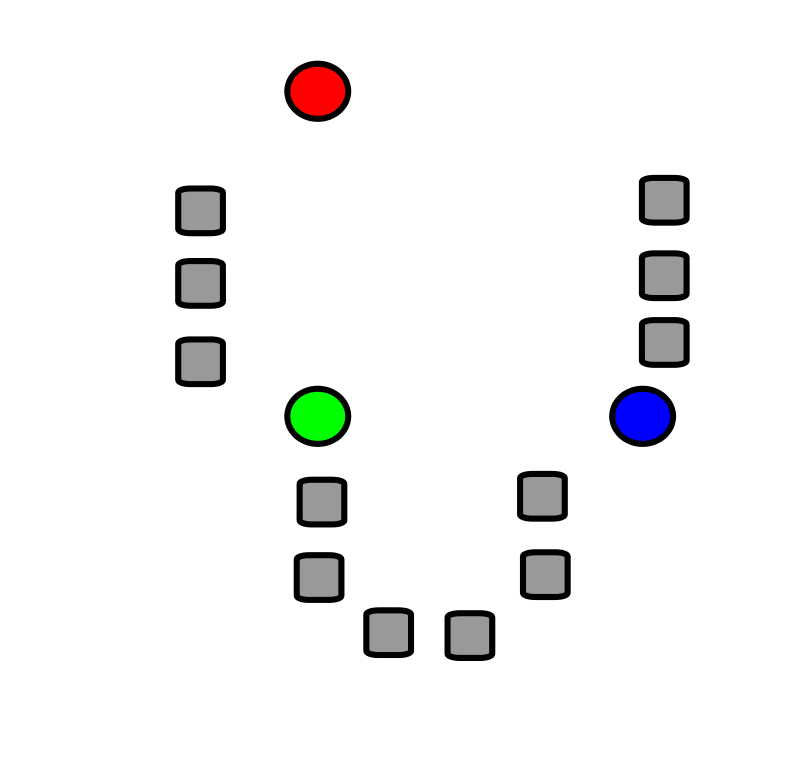
\includegraphics[width=0.5\textwidth]{1.png}
    \caption{Исходные точки и случайно выбранные начальные центры}
\end{figure}

\begin{figure}[H]
    \centering
    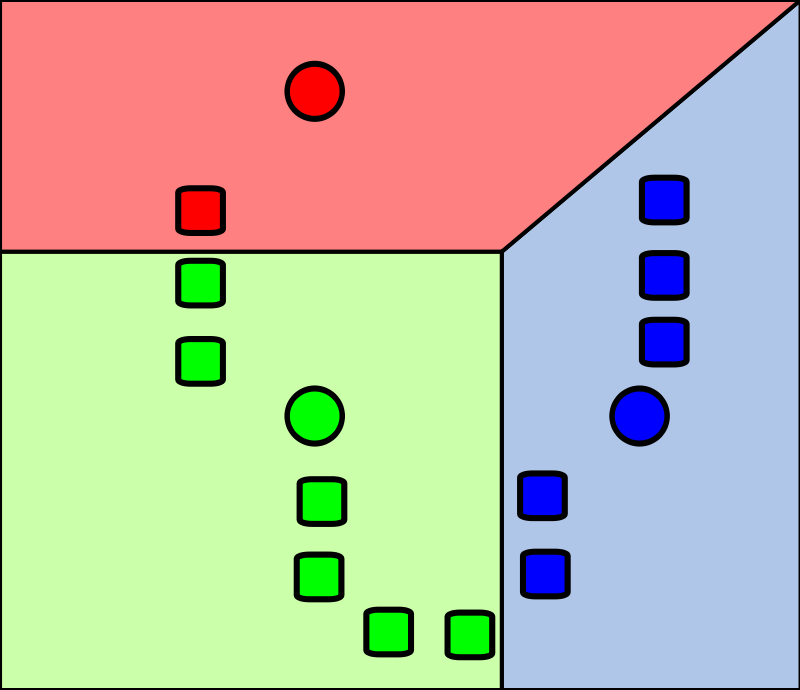
\includegraphics[width=0.5\textwidth]{2.png}
    \caption{Точки, отнесённые к начальным центрам}
\end{figure}

\begin{figure}[H]
    \centering
    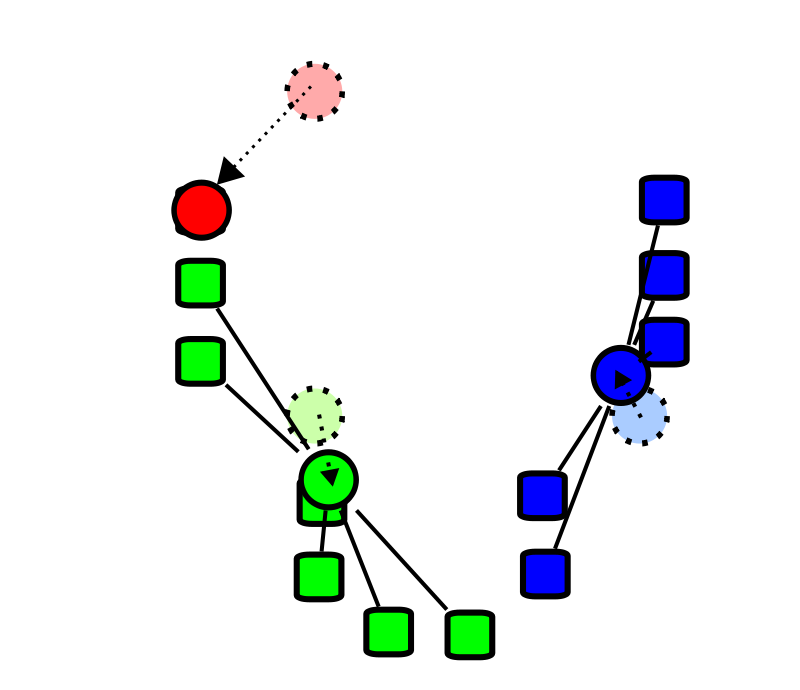
\includegraphics[width=0.5\textwidth]{3.png}
    \caption{Вычисление новых центров кластеров}
\end{figure}

\begin{figure}[H]
    \centering
    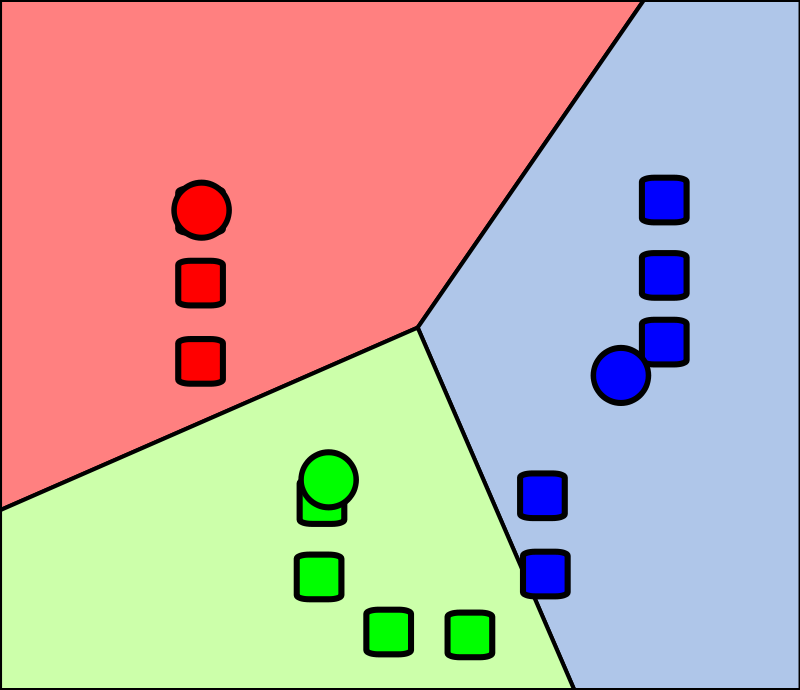
\includegraphics[width=0.5\textwidth]{4.png}
    \caption{Точки, отнесённые к новым центрам}
\end{figure}

Предыдущие шаги, за исключением первого, повторяются, пока алгоритм не сойдётся.

\subsubsection{Проблемы метода}
На вход алгоритма должно подаваться количество кластеров.
Есть два способа выбора количества кластеров:
\begin{enumerate}
    \item Экспертный метод (domain knowledge). Выбор количества кластеров будет зависеть от знания о предметной области.
    \item Метод локтя (elbow method). Можно обучить модель используя несколько вариантов количества кластеров, измерить сумму квадратов внутрикластерных расстояний и выбрать тот вариант, при котором данное расстояние перестанет существенно уменьшаться.
\end{enumerate}

Так же не гарантируется достижение глобального минимума суммарного квадратичного отклонения $J$, а только одного из локальных минимумов. И результат зависит от выбора исходных центров кластеров, их оптимальный выбор неизвестен.

\subsection{DBSCAN}
Основанная на плотности пространственная кластеризация для приложений с шумами (Density-based spatial clustering of applications with noise, \\DBSCAN) -- алгоритм кластеризации, основанной на плотности -- если дан набор точек в некотором пространстве, алгоритм группирует вместе точки, которые тесно расположены, помечая как выбросы точки, которые находятся одиноко в областях с малой плотностью (ближайшие соседи которых лежат далеко) \cite{dbscan}.

Рассмотрим набор точек в некотором пространстве, требующий кластеризации. Для выполнения кластеризации DBSCAN точки делятся на основные точки, достижимые по плотности точки и выпадающие следующим образом:
\begin{enumerate}
    \item Точка p является основной точкой, если по меньшей мере $m$ точек находятся на расстоянии, не превосходящем 
    $\epsilon$  ($\epsilon$ является максимальным радиусом соседства от $p$), до неё (включая саму точку $p$). Говорят, что эти точки достижимы прямо из $p$.

    \item Точка $q$ прямо достижима из $p$, если точка $q$ находится на расстоянии, не большем 
    $\epsilon$ , от точки $p$ и $p$ должна быть основной точкой.

    \item Точка $q$ достижима из $p$, если имеется путь $p_1 = 1, \dots, p_n = q$, где
    каждая точка $p_{i + 1}$ достижима прямо из $p_i$ 
    (все точки на пути должны быть основными, за исключением $q$).

    \item Все точки, не достижимые из основных точек, считаются выбросами.
\end{enumerate}

Теперь, если $p$ является основной точкой, то она формирует кластер вместе со всеми точками (основными или неосновными), достижимые из этой точки. Каждый кластер содержит по меньшей мере одну основную точку. Неосновные точки могут быть частью кластера, но они формируют его «край», поскольку не могут быть использованы для достижения других точек.

\begin{figure}[H]
    \centering
    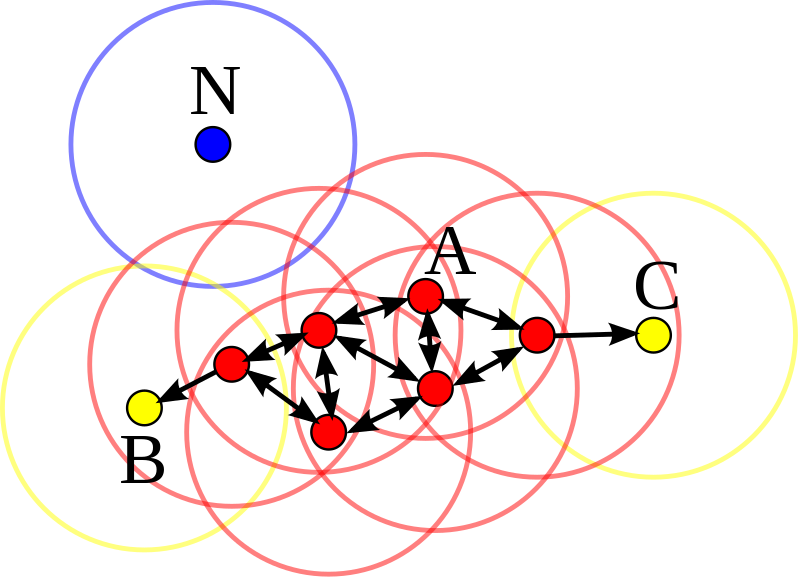
\includegraphics[width=0.5\textwidth]{5.png}
    \caption{Пример диаграммы с $m = 4$}
\end{figure}

Точка A и другие красные точки являются основными точками, поскольку область с радиусом 
$\epsilon$, окружающая эти точки, содержит по меньшей мере 4 точки (включая саму точку). Поскольку все они достижимы друг из друга, точки образуют один кластер. Точки $B$ и $C$ основными не являются, но достижимы из $A$ (через другие основные точки), и также принадлежат кластеру. Точка $N$ является точкой шума, она не является ни основной точкой, ни доступной прямо.

Достижимость не является симметричным отношением, поскольку, по определению, никакая точка не может быть достигнута из неосновной точки, независимо от расстояния (так что неосновная точка может быть достижимой, но ничто не может быть достигнуто из неё). Поэтому дальнейшее понятие связности необходимо для формального определения области кластеров, найденных алгоритмом DBSCAN. Две точки $p$ и $q$ связаны по плотности, если имеется точка $o$, такая что и $p$, и $q$ достижимы из o. Связность по плотности является симметричной.

Тогда кластер удовлетворяет двум свойствам:

\begin{enumerate}
    \item Все точки в кластере попарно связны по плотности.
    \item Если точка достижима по плотности из какой-то точки кластера, она также принадлежит кластеру.
\end{enumerate}

\subsubsection{Алгоритм}
DBSCAN требует задания двух параметров: 
$\epsilon$ и минимального числа точек, которые должны образовывать плотную область $m$. Алгоритм начинается с произвольной точки, которая ещё не просматривалась. Выбирается 
$\epsilon$-окрестность точки и, если она содержит достаточно много точек, образуется кластер, в противном случае точка помечается как шум. Заметим, что эта точка может быть позже найдена в 
$\epsilon$-окрестности другой точки и включена в какой-то кластер.

Если точка найдена как плотная точка кластера, её 
$\epsilon$-окрестность также является частью этого кластера. Следовательно, все точки, найденные в 
$\epsilon$-окрестности этой точки, добавляются к кластеру. Этот процесс продолжается, пока не будет найден связный по плотности кластер. Затем выбирается и обрабатывается новая непосещённая точка, что ведёт к обнаружению следующего кластера или шума.

DBSCAN может быть использован с любой функцией расстояния (а так же с функцией похожести или логическим условием). Функция расстояния может поэтому рассматриваться как дополнительный параметр.

\subsubsection{Преимущества и недостатки}
Преимущества:
\begin{enumerate}
    \item DBSCAN не требует спецификации числа кластеров в данных априори в отличие от метода k-средних.
    \item DBSCAN может найти кластеры произвольной формы. Он может найти даже кластеры полностью окружённые (но не связанные с) другими кластерами. Благодаря параметру MinPts уменьшается так называемый эффект одной связи (связь различных кластеров тонкой линией точек).
    \item DBSCAN имеет понятие шума и устойчив к выбросам.
    \item DBSCAN требует лишь двух параметров и большей частью нечувствителен к порядку точек в базе данных. (Однако, точки, находящиеся на границе двух различных кластеров могут оказаться в другом кластере, если изменить порядок точек, а назначение кластеров единственно с точностью до изоморфизма).
    \item DBSCAN разработан для применения с базами данных, которые позволяют ускорить запросы в диапазоне значений, например, с помощью R*-дерева.
    \item Параметры $m$ и $\epsilon$ могут быть установлены экспертами в рассматриваемой области, если данные хорошо понимаются.
\end{enumerate}

Недостатки:
\begin{enumerate}
    \item DBSCAN не полностью однозначен — краевые точки, которые могут быть достигнуты из более чем одного кластера, могут принадлежать любому из этих кластеров, что зависит от порядка просмотра точек. Для большинства наборов данных эти ситуации возникают редко и имеют малое влияние на результат кластеризации -- основные точки и шум DBSCAN обрабатывает однозначно. DBSCAN является вариантом, который трактует краевые точки как шум и тем самым достигается полностью однозначный результат, а также более согласованная статистическая интерпретация связных по плотности компонент.
    \item Качество DBSCAN зависит от измерения расстояния. Наиболее часто используемой метрикой расстояний является евклидова метрика. Особенно для кластеризации данных высокой размерности эта метрика может оказаться почти бесполезной ввиду так называемого «проклятия размерности», что делает трудным делом нахождение подходящего значения 
    $\epsilon$. Этот эффект, однако, присутствует в любом другом алгоритме, основанном на евклидовом расстоянии.

    \item DBSCAN не может хорошо кластеризовать наборы данных с большой разницей в плотности, поскольку не удается выбрать приемлемую для всех кластеров комбинацию $m - \epsilon$.
    \item Если данные и масштаб не вполне хорошо поняты, выбор осмысленного порога расстояния 
    $\epsilon$  может оказаться трудным.
\end{enumerate}

\conclusion
Таким образом, обучение без учителя -- это процесс обучения модели на основе неразмеченных данных, где нет известных меток или целевых переменных. В этом случае модель ищет скрытые структуры и закономерности в данных, чтобы создать представление или кластеризацию данных.

Преимуществами данного метода обучения являются:
\begin{enumerate}
    \item Извлечение скрытых структур. Обучение без учителя позволяет модели извлекать скрытые структуры и паттерны из данных, что может быть полезно для обнаружения новых знаний и понимания данных.
    \item Работа с большими объемами данных. Обучение без учителя может быть эффективным при работе с большими объемами данных, поскольку нет необходимости размечать каждый пример.
    \item Автоматическое обучение. Обучение без учителя позволяет модели самостоятельно находить паттерны и структуры в данных, без необходимости вручную определять правильные ответы.
\end{enumerate}

Недостатки:
\begin{enumerate}
    \item Неопределенность результатов. Результаты обучения без учителя могут быть менее интерпретируемыми и требуют дополнительного анализа и проверки.
    \item Трудность оценки. Оценка качества модели в обучении без учителя может быть сложной, поскольку нет явных правильных ответов для сравнения.
    \item Необходимость предварительной обработки данных. В обучении без учителя может потребоваться предварительная обработка данных для удаления шума или выбросов, что может быть трудоемким процессом.
\end{enumerate}
https://masters.donntu.ru/2006/kita/chvala/library/N3.pdf
\begin{thebibliography}{10}
    \bibitem{hebb1}
    Короткий С. Нейронные сети: обучение без учителя [Электронный ресурс] -- URL: https://masters.donntu.ru/2006/kita/chvala/library/N3.pdf. (Дата обращения 11.01.2024). Загл. с экр. Яз. рус.

    \bibitem{hebb2}
    Обучение Хебба: простыми словами о принципах, алгоритме и применении в нейронных сетях [Электронный ресурс]. -- URL: https://skine.ru/articles/1511/
    (Дата обращения 11.01.2024). Загл. с экр. Яз. рус.

    \bibitem{cluster}
    Горбаченко В. И. Самоорганизация в нейронных сетях [Электронный ресурс] //Научно-исследовательский центр самоорганизации и развития систем.--2018. -- URL: http://gorbachenko.self-organization.ru/articles/Self-organizing_map.pdf. (Дата обращения 11.01.2024). Загл. с экр. Яз. рус.

    \bibitem{kmean1}
    Алгоритм кластеризации K-средних [Электронный ресурс]. -- URL: https://skine.ru/articles/1511/
    (Дата обращения 11.01.2024). Загл. с экр. Яз. рус.

    \bibitem{kmean2}
    Метод k-средних [Электронный ресурс]. -- URL: https://ru.wikipedia.org/wiki/Метод_k-средних
    (Дата обращения 11.01.2024). Загл. с экр. Яз. рус.

    \bibitem{dbscan}
    DBSCAN [Электронный ресурс]. -- URL: https://ru.wikipedia.org/wiki/DBSCAN
    (Дата обращения 11.01.2024). Загл. с экр. Яз. рус.
\end{thebibliography}

\end{document}